%% Baseado no arquivo: 
%% abtex2-modelo-trabalho-academico.tex, v-1.9.6 laurocesar
%% by abnTeX2 group at http://www.abntex.net.br/ 
%% Adaptado para um modelo dssse TCC (Graduação)

% ------------------------------------------------------------------------
% ------------------------------------------------------------------------
% abnTeX2: Modelo de Trabalho Academico (tese de doutorado, dissertacao de
% mestrado e trabalhos monograficos em geral) em conformidade com 
% ABNT NBR 14724:2011: Informacao e documentacao - Trabalhos academicos -
% Apresentacao
% ------------------------------------------------------------------------
% ------------------------------------------------------------------------

\documentclass[
	% -- opções da classe memoir --
	12pt,				% tamanho da fonte
	openright,			% capítulos começam em pág ímpar (insere página vazia caso preciso)
	oneside,			% para impressão em recto e verso. Oposto a oneside
	a4paper,			% tamanho do papel. 
	% -- opções da classe abntex2 --
	%chapter=TITLE,		% títulos de capítulos convertidos em letras maiúsculas
	%section=TITLE,		% títulos de seções convertidos em letras maiúsculas
	%subsection=TITLE,	% títulos de subseções convertidos em letras maiúsculas
	%subsubsection=TITLE,% títulos de subsubseções convertidos em letras maiúsculas
	% -- opções do pacote babel --
	english,			% idioma adicional para hifenização
	%french,				% idioma adicional para hifenização
	%spanish,			% idioma adicional para hifenização
	brazil				% o último idioma é o principal do documento
	]{abntex2}

% ---
% Pacotes básicos 
% ---
\usepackage{lmodern}			% Usa a fonte Latin Modern			
\usepackage[T1]{fontenc}		% Selecao de codigos de fonte.
\usepackage[utf8]{inputenc}		% Codificacao do documento (conversão automática dos acentos)
\usepackage{lastpage}			% Usado pela Ficha catalográfica
\usepackage{indentfirst}		% Indenta o primeiro parágrafo de cada seção.
\usepackage{color}				% Controle das cores
\usepackage{graphicx}			% Inclusão de gráficos
\usepackage{microtype} 			% para melhorias de justificação
\usepackage{float}				% para controle de posicionamento de figuras e tabelas
\usepackage{pdfpages} 			% para inclusão de PDFs
% ---
		

% ---
% Pacotes de citações
% ---
\usepackage[brazilian,hyperpageref]{backref}	 % Paginas com as citações na bibl
\usepackage[alf]{abntex2cite}	% Citações padrão ABNT

% --- 
% CONFIGURAÇÕES DE PACOTES
% --- 

% ---
% Configurações do pacote backref
% Usado sem a opção hyperpageref de backref
\renewcommand{\backrefpagesname}{%Citado na(s) página(s):~
}
% Texto padrão antes do número das páginas
\renewcommand{\backref}{}
% Define os textos da citação
\renewcommand*{\backrefalt}[4]{
	%\ifcase #1 %
	%	Nenhuma citação no texto.%
	%\or
	%	Citado na página #2.%
	%\else
	%	Citado #1 vezes nas páginas #2.%
	%\fi
    }%
% ---

% ---
% Informações de dados para CAPA e FOLHA DE ROSTO
% ---
\titulo{Jogo de Xadrez com Manipuladores Robóticos}
\autor{Rafael Dias Campos}
\local{Belo Horizonte}
\data{2022}
\orientador{Ramon da Cunha Lopes}
\instituicao{%
  Centro Federal de Educação Tecnológica de Minas Gerais -- CEFET-MG
  \par
  Departamento de Computação
  \par
  Curso de Engenharia da Computação
  }
\tipotrabalho{Monografia (Graduação)}
% O preambulo deve conter o tipo do trabalho, o objetivo, 
% o nome da instituição e a área de concentração 
\preambulo{Trabalho de Conclusão de Curso apresentado ao Curso
de Engenharia de Computação do Centro Federal de
Educação Tecnológica de Minas Gerais, como requisito
parcial para a obtenção do título de Bacharel em
Engenharia de Computação.}
% ---


% ---
% Configurações de aparência do PDF final

% alterando o aspecto da cor azul
\definecolor{blue}{RGB}{41,5,195}

% informações do PDF
\makeatletter
\hypersetup{
     	%pagebackref=true,
		pdftitle={\@title}, 
		pdfauthor={\@author},
    	pdfsubject={\imprimirpreambulo},
	    pdfcreator={LaTeX with abnTeX2},
		pdfkeywords={abnt}{latex}{abntex}{abntex2}{trabalho acadêmico}, 
		colorlinks=true,       		% false: boxed links; true: colored links
    	linkcolor=blue,          	% color of internal links
    	citecolor=blue,        		% color of links to bibliography
    	filecolor=magenta,      		% color of file links
		urlcolor=blue,
		bookmarksdepth=4
}
\makeatother
% --- 

% --- 
% Espaçamentos entre linhas e parágrafos 
% --- 

% O tamanho do parágrafo é dado por:
\setlength{\parindent}{1.3cm}

% Controle do espaçamento entre um parágrafo e outro:
\setlength{\parskip}{0.2cm}  % tente também \onelineskip

% ---
% compila o indice
% ---
\makeindex
% ---

% ----
% Início do documento
% ----
\begin{document}

% Seleciona o idioma do documento (conforme pacotes do babel)
%\selectlanguage{english}
%\selectlanguage{brazil}

% Retira espaço extra obsoleto entre as frases.
\frenchspacing 

% ----------------------------------------------------------
% ELEMENTOS PRÉ-TEXTUAIS
% ----------------------------------------------------------



%% Baseado no arquivo: 
%% abtex2-modelo-trabalho-academico.tex, v-1.9.6 laurocesar
%% by abnTeX2 group at http://www.abntex.net.br/ 
%% Adaptado para um modelo de TCC (Graduação)

% ---
% Capa
% ---
\imprimircapa
% ---

% ---
% Folha de rosto
% (o * indica que haverá a ficha bibliográfica)
% ---
\imprimirfolhaderosto*
% ---

% ---
% Inserir a ficha bibliografica
% ---

% Isto é um exemplo de Ficha Catalográfica, ou ``Dados internacionais de
% catalogação-na-publicação''. Você pode utilizar este modelo como referência. 
% Porém, provavelmente a biblioteca da sua universidade lhe fornecerá um PDF
% com a ficha catalográfica definitiva após a defesa do trabalho. Quando estiver
% com o documento, salve-o como PDF no diretório do seu projeto e substitua todo
% o conteúdo de implementação deste arquivo pelo comando abaixo:
%
% \begin{fichacatalografica}
%     
% \end{fichacatalografica}

\begin{fichacatalografica}
~
%\includepdf{fig_ficha_catalografica.pdf}
% 	\sffamily
% 	\vspace*{\fill}					% Posição vertical
% 	\begin{center}					% Minipage Centralizado
% 	\fbox{\begin{minipage}[c][8cm]{13.5cm}		% Largura
% 	\small
% 	\imprimirautor
% 	%Sobrenome, Nome do autor
	
% 	\hspace{0.5cm} \imprimirtitulo  / \imprimirautor. --
% 	\imprimirlocal, \imprimirdata-
	
% 	\hspace{0.5cm} \pageref{LastPage} p. : il. (algumas color.) ; 30 cm.\\
	
% 	\hspace{0.5cm} \imprimirorientadorRotulo~\imprimirorientador\\
	
% 	\hspace{0.5cm}
% 	\parbox[t]{\textwidth}{\imprimirtipotrabalho~--~\imprimirinstituicao,
% 	\imprimirdata.}\\
	
% 	\hspace{0.5cm}
% 		1. Palavra-chave1.
% 		2. Palavra-chave2.
% 		2. Palavra-chave3.
% 		I. Orientador.
% 		II. Universidade xxx.
% 		III. Faculdade de xxx.
% 		IV. Título 			
% 	\end{minipage}}
% 	\end{center}
\end{fichacatalografica}
% ---

% % ---
% % Inserir errata
% % ---
% \begin{errata}
% Elemento opcional da \citeonline[4.2.1.2]{NBR14724:2011}. Exemplo:

% \vspace{\onelineskip}

% FERRIGNO, C. R. A. \textbf{Tratamento de neoplasias ósseas apendiculares com
% reimplantação de enxerto ósseo autólogo autoclavado associado ao plasma
% rico em plaquetas}: estudo crítico na cirurgia de preservação de membro em
% cães. 2011. 128 f. Tese (Livre-Docência) - Faculdade de Medicina Veterinária e
% Zootecnia, Universidade de São Paulo, São Paulo, 2011.

% \begin{table}[htb]
% \center
% \footnotesize
% \begin{tabular}{|p{1.4cm}|p{1cm}|p{3cm}|p{3cm}|}
%   \hline
%    \textbf{Folha} & \textbf{Linha}  & \textbf{Onde se lê}  & \textbf{Leia-se}  \\
%     \hline
%     1 & 10 & auto-conclavo & autoconclavo\\
%    \hline
% \end{tabular}
% \end{table}

% \end{errata}
% ---

% ---
% Inserir folha de aprovação
% ---


%
\begin{folhadeaprovacao}

  \begin{center}
    Espaço destinado à folha de aprovação
%após aprovação, insira a cópia da folha de aprovação por meio do comando:
% \includepdf{folhadeaprovacao_final.pdf}
  \end{center}
  
\end{folhadeaprovacao}
% ---

% ---
% Dedicatória
% ---
\begin{dedicatoria}
   \vspace*{\fill}
   \centering
   \noindent
   \textit{Dedico este trabalho aos alunos(as) do CEFET-MG.} \vspace*{\fill}
\end{dedicatoria}
% ---

% ---
% Agradecimentos
% ---
\begin{agradecimentos}
Agradeço ao Latex e às pessoas que contribuiram com o desenvolvimento do Abntex2 por facilitarem a vida dos graduandos.
\end{agradecimentos}
% ---

% ---
% Epígrafe
% ---
\begin{epigrafe}
    \vspace*{\fill}
	\begin{flushright}
		\textit{``As pessoas costumam dizer que a motivação não dura sempre. Bem, nem o efeito do banho, por isso recomenda-se diariamente.''\\
		(Zig Ziglar)}
	\end{flushright}
\end{epigrafe}
% ---

% ---
% RESUMOS
% ---

% resumo em português
\setlength{\absparsep}{18pt} % ajusta o espaçamento dos parágrafos do resumo
\begin{resumo}
Neste trabalho será realizado o controle digital de dois manipuladores robóticos para a movimentação de peças de Xadrez. 

Inicialmente, será realizado o controle de um manipulador para possibilitar que um ser-humano jogue uma partida com o computador.
Em seguida, o segundo manipulador será controlado para que duas pessoas joguem uma partida entre si.

 \textbf{Palavras-chave}: Manipuladores Robóticos. Controle Digital. Xadrez
\end{resumo}

% resumo em inglês
\begin{resumo}[Abstract]
 \begin{otherlanguage*}{english}
   In this thesis, will be implemented the digital control of two robotic arms to move chess pieces.

   Initially, a single arm will be controlled in order to allow a human player to play against the computer.
   Further on, the second arm will be controlled so that two human players can play against each other.

   \vspace{\onelineskip}
 
   \noindent 
   \textbf{Keywords}: Robotic Arms. Digital Control. Chess.
 \end{otherlanguage*}
\end{resumo}


% ---

% ---
% inserir lista de ilustrações
% ---
\pdfbookmark[0]{\listfigurename}{lof}
\listoffigures*
\cleardoublepage
% ---

% ---
% inserir lista de tabelas
% ---
\pdfbookmark[0]{\listtablename}{lot}
\listoftables*
\cleardoublepage
% ---

% ---
% inserir lista de abreviaturas e siglas
% ---
\begin{siglas}
  \item[CEFET-MG] Centro Federal de Educação Tecnológica de Minas Gerais
  \item[STEM] \textit{Science, Technology, Engineering and Mathematics} [Ciência, Tecnologia, Engenharia e Matemática]
\end{siglas}
% ---

% ---
% inserir lista de símbolos
% ---
\begin{simbolos}
  \item[$ \Gamma $] Letra grega Gama
  \item[$ \Lambda $] Lambda
  \item[$ \zeta $] Letra grega minúscula zeta
  \item[$ \in $] Pertence
\end{simbolos}
% ---

% ---
% inserir o sumario
% ---
\pdfbookmark[0]{\contentsname}{toc}
\tableofcontents*
\cleardoublepage
% ---

% ----------------------------------------------------------
% ELEMENTOS TEXTUAIS
% ----------------------------------------------------------
\textual

% ----------------------------------------------------------
% Como o documento será grande, sugiro dividir em diversos arquivos, um para cada capítulo.
% ----------------------------------------------------------


\chapter[Introdução]{Introdução}
\label{cap:introducao}

Atualmente, existe uma grande procura por funcionários especializados em Tecnologia da Informação (TI) e áreas similares,
sendo percebida no mundo todo uma grande carência de profissionais qualificados para atuar nessas áreas \cite{shortage_of_workers}.

Com base nisso, foi proposto realizar o desenvolvimento de uma plataforma que utilize recursos computacionais passível de ser utilizada para demonstrar conceitos nas áreas de computação, elétrica e controle.
Para aumentar o interesse por ela foi definido que deve permitir que os participantes joguem uma partida de Xadrez.

Correlacionando essas ideias, foi decidido implementar um jogo de Xadrez que pode ser jogado através de braços robóticos.

\section[Motivação]{Motivação}

Considerando a carência de profissionais de TI no mercado, torna-se importante a busca por formas de incentivar o aprendizado e a busca por conhecimento por parte dos jovens.
Para tornar o aprendizado mais atrativo e divertido, foi feita a incorporação de um jogo no projeto proposto.
Finalmente, foi decidido que o projeto deveria usar elementos da robótica, visto que pesquisas demonstram que seu uso em atividades com crianças consegue influenciar positivamente o desenvolvimento de habilidades da área de STEM \cite{technology_for_stem}.

\section[Objetivos]{Objetivos}

Este trabalho visa desenvolver um sistema de controle de manipuladores robóticos que permitam que dois jogadores participem em uma partida de Xadrez.

Caso haja disponibilidade de tempo, o sistema também possibilitará que o jogo seja jogado por um jogador humano e um computador ou jogador humano através da Internet.

\section[Relevância]{Relevância}

Com o desenvolvimento dessa plataforma, será possível demonstrar conceitos de computação, elétrica e controle de forma prática e divertida.
Ela pode ser facilmente transportada para diferentes locais e apresentada em eventos, como feiras de ciências, por exemplo.
Dessa forma, ela pode promover e instigar a busca por conhecimento, além de atrair futuros profissionais para a área de TI.

\chapter[Planejamento]{Planejamento}
\label{cap:planejamento}

Nesta seção, será descrito o planejamento do projeto.

\section[Escolha do equipamento]{Escolha do equipamento}

Para o desenvolvimento do projeto, foram disponibilizados, pela instituição CEFET-MG, dois manipuladores robóticos e diversos dispositivos que podem ser utilizados para seu controle.

\subsection[Manipuladores]{Manipuladores}

Os principais elementos deste trabalho são os manipuladores robóticos, portanto foi feito inicialmente um estudo sobre seu funcionamento e sobre como podem ser controlados.

Os manipuladores disponibilizados possuem diferenças físicas entre si, portanto o controle de cada um deles deve ser programado de forma independente.
Para diferenciá-los, serão denominados Manipulador Azul e Manipulador Preto.
A seguir, serão descritos os principais aspectos de cada um deles.

\begin{figure}[H]
    \begin{minipage}{.5\textwidth}
        \centering
        \caption{Manipulador Robótico Azul}
        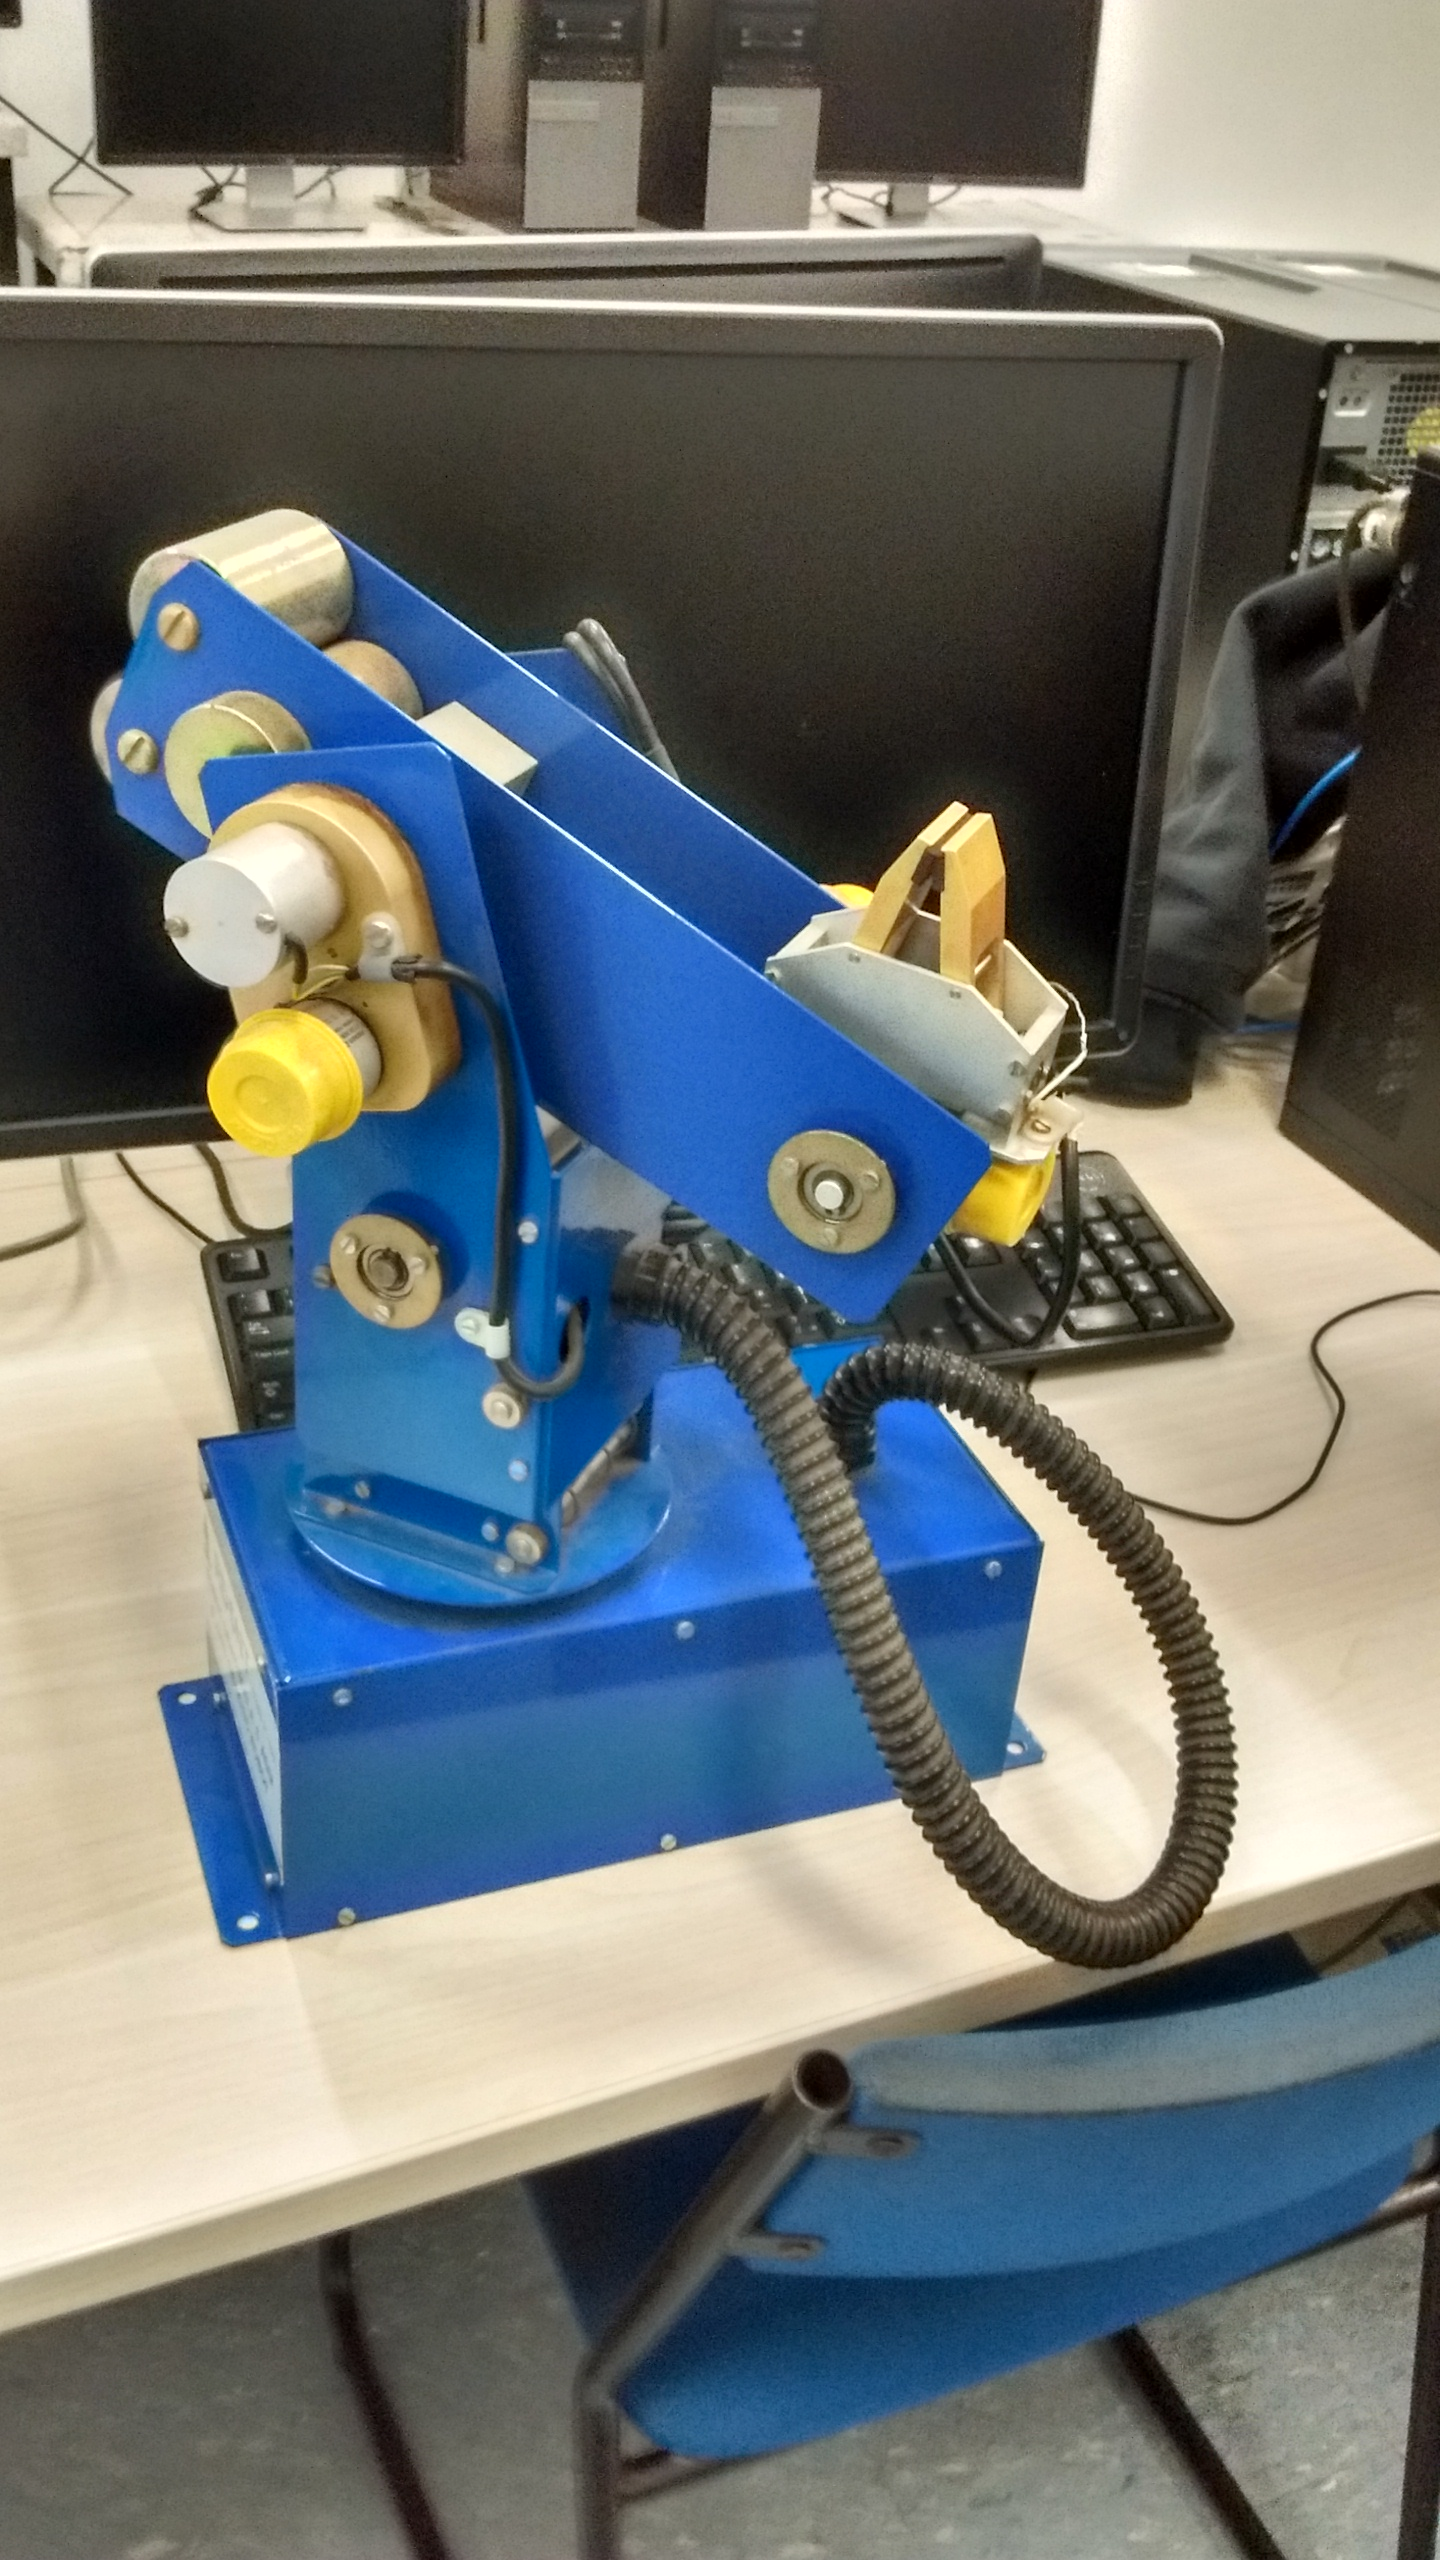
\includegraphics[keepaspectratio=true, width=0.9\linewidth]
            {img/foto-manipulador-azul.jpg}
        \fonte{http://arquivo.eng.br/robotica}
        \label{fig:fotoManipuladorAzul}
    \end{minipage}%
    \begin{minipage}{.5\textwidth}
        \centering
        \caption{Manipulador Robótico Preto}
        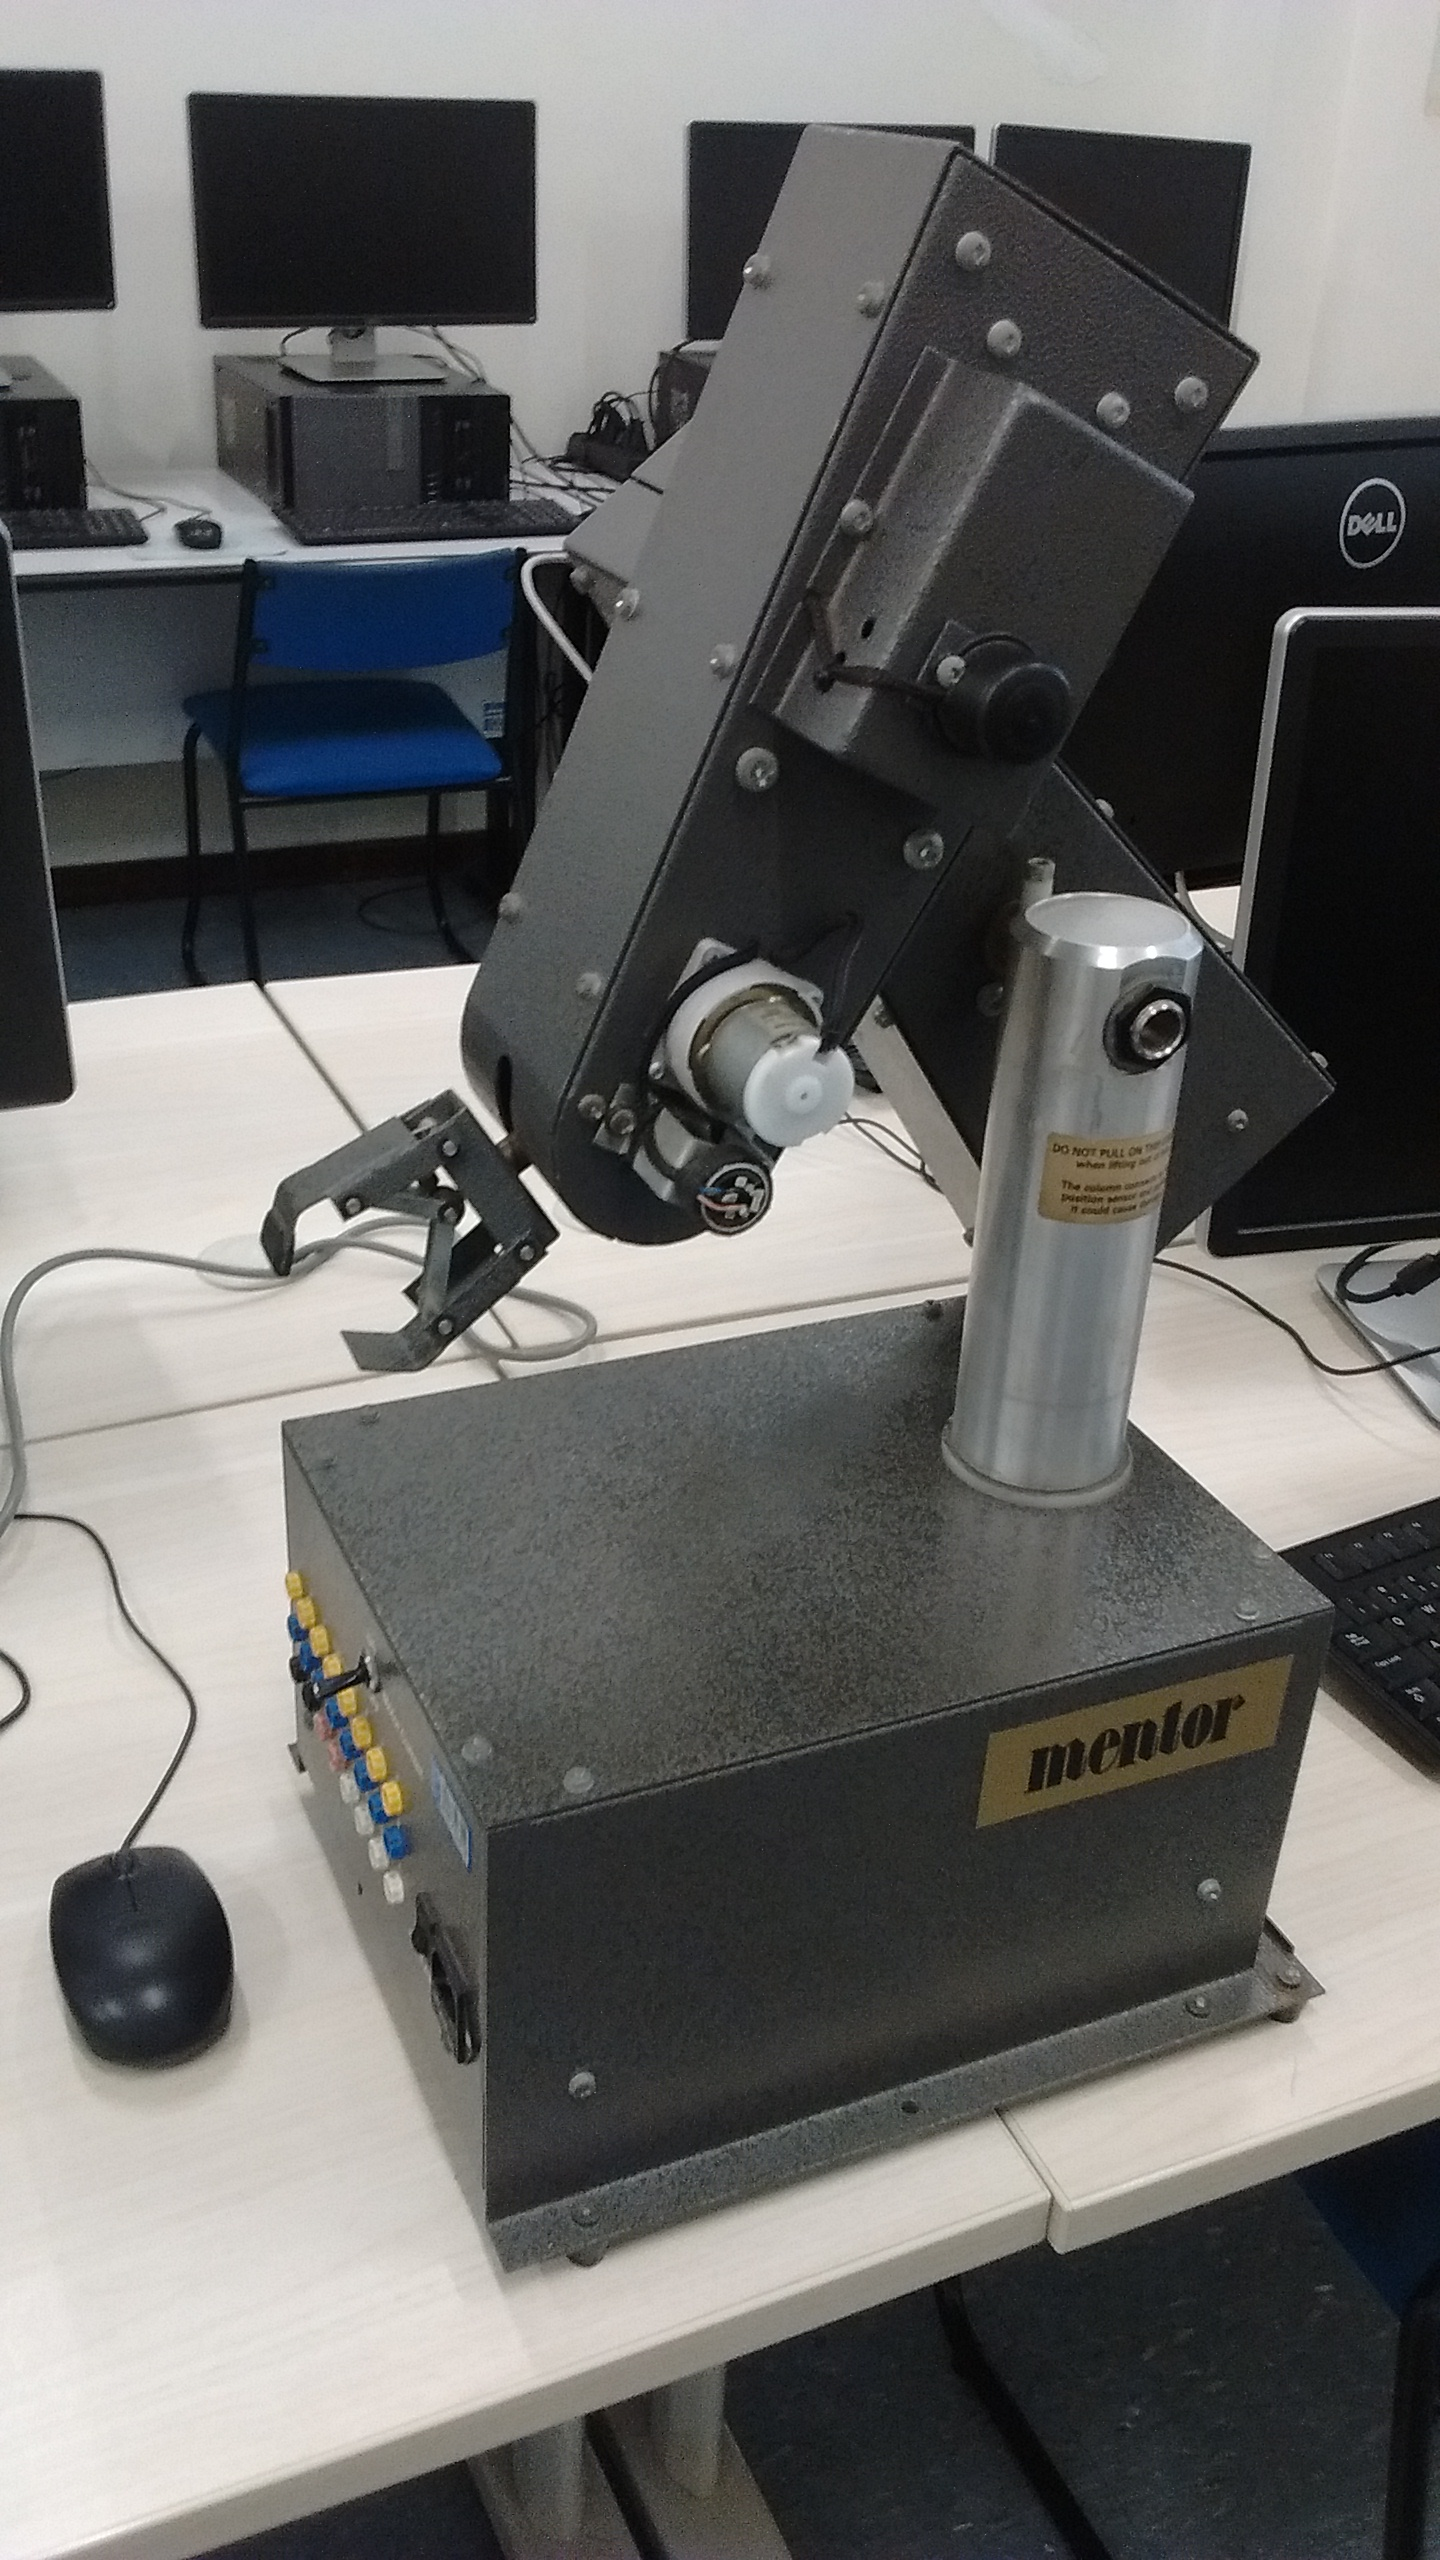
\includegraphics[keepaspectratio=true, width=0.9\linewidth]
            {img/foto-manipulador-preto.jpg}
        \fonte{http://arquivo.eng.br/robotica}
        \label{fig:fotoManipuladorPreto}
    \end{minipage}
\end{figure}

\subsection[Manete para os jogadores]{Manete para os jogadores}

Para que os jogadores possam interagir com os manipuladores, foi utilizado uma manete que possui dois \textit{joysticks} e um botão integrado a cada \textit{joystick}.
Cada jogador possui uma manete para mover seu manipulador nos eixos X e Y, e selecionar a peça que deseja mover.

\begin{figure}[H]
    \centering
    \caption{Manete para os jogadores}
    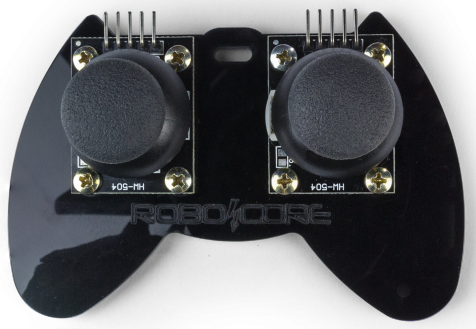
\includegraphics[keepaspectratio=true, width=0.5\textwidth]
    	{img/foto-controle-jogadores.png}
    \fonte{https://www.robocore.net/acessorios-robocore/controle-batpad}
    \label{fig:fotoManeteJogadores}
\end{figure}

\subsection[Microcontrolador]{Microcontrolador}

Para realizar a leitura dos dados das manetes e enviar os comandos para os manipuladores, foi utilizado um microcontrolador Arduino Uno.
Este dispositivo deve receber sinais analógicos provenientes dos \textit{joysticks}, receber sinais digitais provenientes dos botões nos controles, receber sinais analógicos que indicam as posições dos manipuladores e enviar sinais digitais do tipo PWM para os motores dos manipuladores.

\begin{figure}[H]
    \centering
    \caption{Microcontrolador Arduino Uno}
    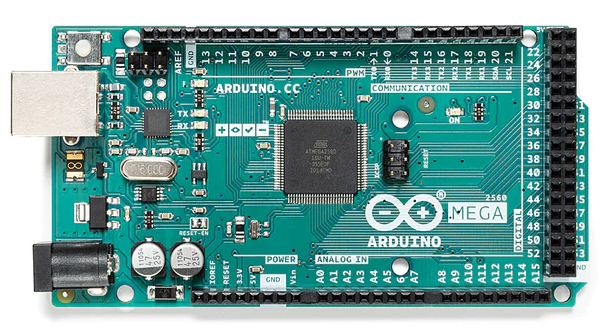
\includegraphics[keepaspectratio=true, width=0.5\textwidth]
    	{img/foto-arduino.png}
    \fonte{https://store-usa.arduino.cc/products/arduino-uno-rev3}
    \label{fig:fotoArduino}
\end{figure}

\section[Projeto do sistema]{Projeto do sistema}

Com todos os equipamentos definidos, foi feito o projeto do sistema, que consiste na definição de como os dispositivos serão interligados e como o sistema irá funcionar.

O microcontrolador Arduino é a base do sistema, pois ele realiza a interligação entre os outros componentes.
As manetes são conectadas ao Arduino por meio de 10 cabos cada, sendo 5 para cada \textit{joystick}, com seu respectivo botão.
Os manipuladores são conectados ao Arduino por meio de 10 cabos cada, sendo 5 para a leitura de cada ângulo dos motores, e 5 para o controle desses.

A montagem do sistema é mostrada na Figura %\ref{fig:montagemSistema}.%

%Inserir figura%




\chapter[Desenvolvimento]{Desenvolvimento}
\label{cap:desenvolvimento}

Após o planejamento do projeto, foi feito o desenvolvimento de cada etapa.
Inicialmente, foi feito o desenvolvimento da placa de controle para poder acionar os motores.
Em seguida, o \textit{software} para ler os dados das manetes e enviar os comandos para a placa de controle foi desenvolvido.

\section[Desenvolvimento da placa de controle]{Desenvolvimento da placa de controle}
\label{sec:desenvolvimentoPlacaControle}

Primeiramente, foi feito o desenvolvimento da placa de controle dos manipuladores, pois é necessária para testar o funcionamento dos motores e do \textit{software} que será desenvolvido.
Para isso, foi necessário definir quais componentes utilizar e como conectá-los.

Conforme descrito na subseção \ref{sub:placaControle}, a placa de controle deve utilizar uma ponte H para o controle de cada junta.
Para isso, foi escolhido o CI L293D, que possui duas pontes H e suporta tensões de 12V.
Como é necessário controlar 6 motores, foram utilizados 3 CI L293D.

Para simplificar o controle e evitar problemas de acionamento duplo das entradas das pontes H, foi utilizado o CI 74LS02 como um inversor lógico.
Dessa forma, a placa de controle possui para cada junta uma entrada de \textit{Enable} para ligar/desligar o acionamento da junta, e uma porta de \textit{Direction} para definir a direção de movimentação dela.
A partir dessas entradas, o CI L293D é acionado e o motor é controlado.
A Figura \ref{fig:esquematicoSimplificado} mostra o esquemático simplificado de um CI L293D e um CI 74LS02.

\begin{figure}[H]
    \centering
    \caption{Esquemático Simplificado de um CI L293D e um CI 74LS02}
    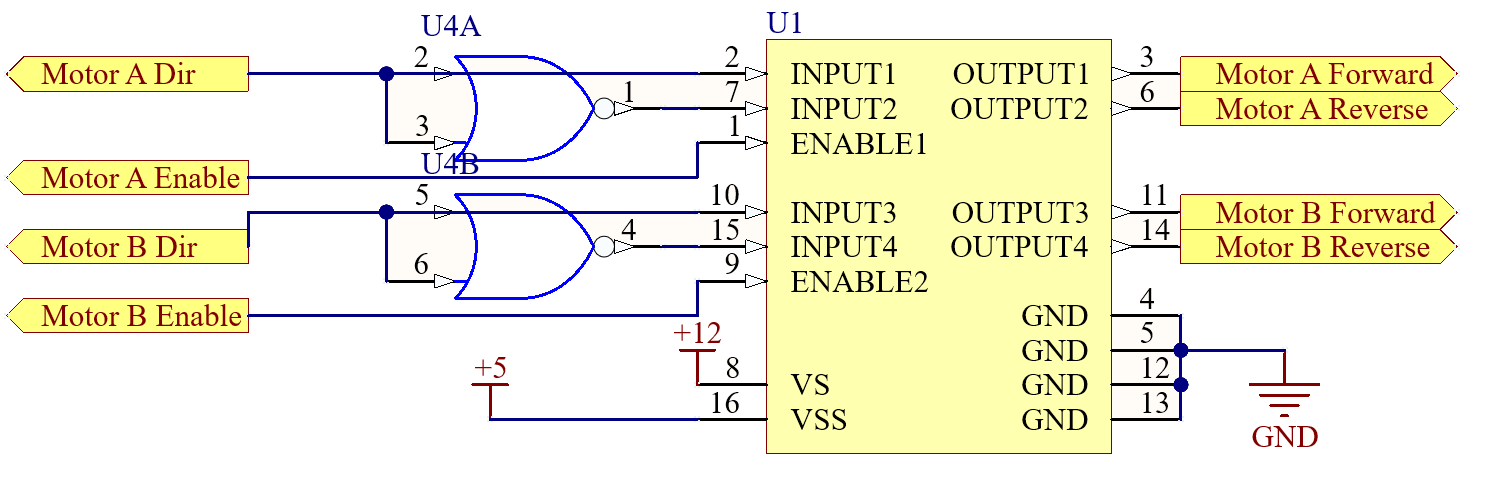
\includegraphics[keepaspectratio=true, width=0.9\textwidth]
    	{img/placa-controle-esquematico-simplificado.png}
    \fonte{Do próprio autor}
    \label{fig:esquematicoSimplificado}
\end{figure}

Com os componentes principais definidos foi feito o desenvolvimento do esquemático da placa de controle com o auxílio do software \textit{Altium Designer}.
O Anexo \ref{anexo:esquematico-placa-controle} mostra o esquemático completo da placa de controle.
Nesse esquemático foram adicionados resistores de \textit{pulldown} para garantir que as entradas dos CI L293D e 74LS02 permaneçam em nível lógico baixo caso não estejam conectadas ao microcontrolador.
Também foram adicionadas \textit{LEDs} para indicar a alimentação de 5V e 12V da placa.

Após o desenvolvimento do esquemático, foi feita a montagem da Placa de Circuito Impresso (PCB), ainda com o auxílio do software \textit{Altium Designer}.
Para isso, os componentes foram posicionados no \textit{layout} da placa, tendo em vista a economia de espaço e a necessidade de manter os componentes próximos para facilitar sua conexão.
Em seguida, as trilhas e vias que realizam a conexão dos componentes foram desenhadas. 
Para permitir a conexão de todos os componentes, foi necessário utilizar uma placa com 2 camadas.
A Figura \ref{fig:placaControleLayout} mostra o \textit{layout} final da placa de controle.

Com o \textit{layout} finalizado, foi feita a produção da PCB de forma manual.
Para isso, o negativo do \textit{layout} foi impresso em uma folha de transparência.
Depois, uma placa de circuito impresso de duas camadas foi cortada no tamanho desejado.

Em seguida, foi feita a transferência do \textit{layout} para a placa.
Para isso, uma fina camada de tinta fotossensível destinada para PCB foi aplicada sobre a placa.
Essa tinta foi pré-curada à 75$^{\circ}$C durante 15 minutos com o auxílio de uma base de aquecimento, para garantir que ela não se descolasse da placa.
Após a pré-cura, a tinta foi exposta à luz ultravioleta por 3 minutos, utilizando a transparência com o \textit{layout} como máscara.
Em seguida, a placa foi submersa em uma solução de carbonato de sódio para realizar a revelação do \textit{layout}.
Após a placa ser revelada, a tinta foi curada à 85$^{\circ}$C durante 30 minutos.

Esse processo de transferência do \textit{layout} foi repetido para a segunda camada da placa.
Em seguida, foi utilizada uma solução de percloreto de ferro para corroer as áreas de cobre que não receberam tinta.
Após a corrosão, a placa foi mergulhada em uma solução de hidróxido de sódio para remover a tinta.

Após a corrosão da PCB, foi feita a perfuração das vias e dos furos para os componentes.
Por fim, foi feita a soldagem dos componentes na placa e a conexão das vias.
A Figura \ref{fig:placaControle} mostra a placa de controle montada.

\begin{figure}[H]
    \begin{minipage}{.5\textwidth}
        \centering
        \caption{Layout da placa de controle}
        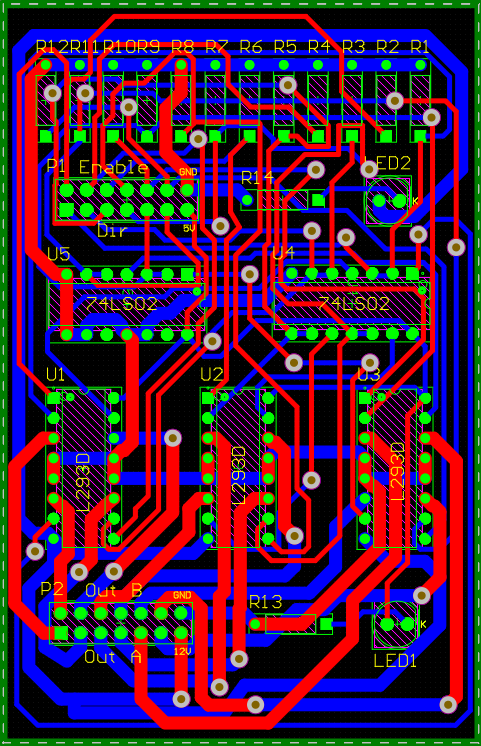
\includegraphics[keepaspectratio=true, width=0.9\linewidth]
            {img/placa-controle-layout.png}
        \fonte{Do próprio autor}
        \label{fig:placaControleLayout}
    \end{minipage}%
    \begin{minipage}{.5\textwidth}
        \centering
        \caption{Placa de controle produzida}
        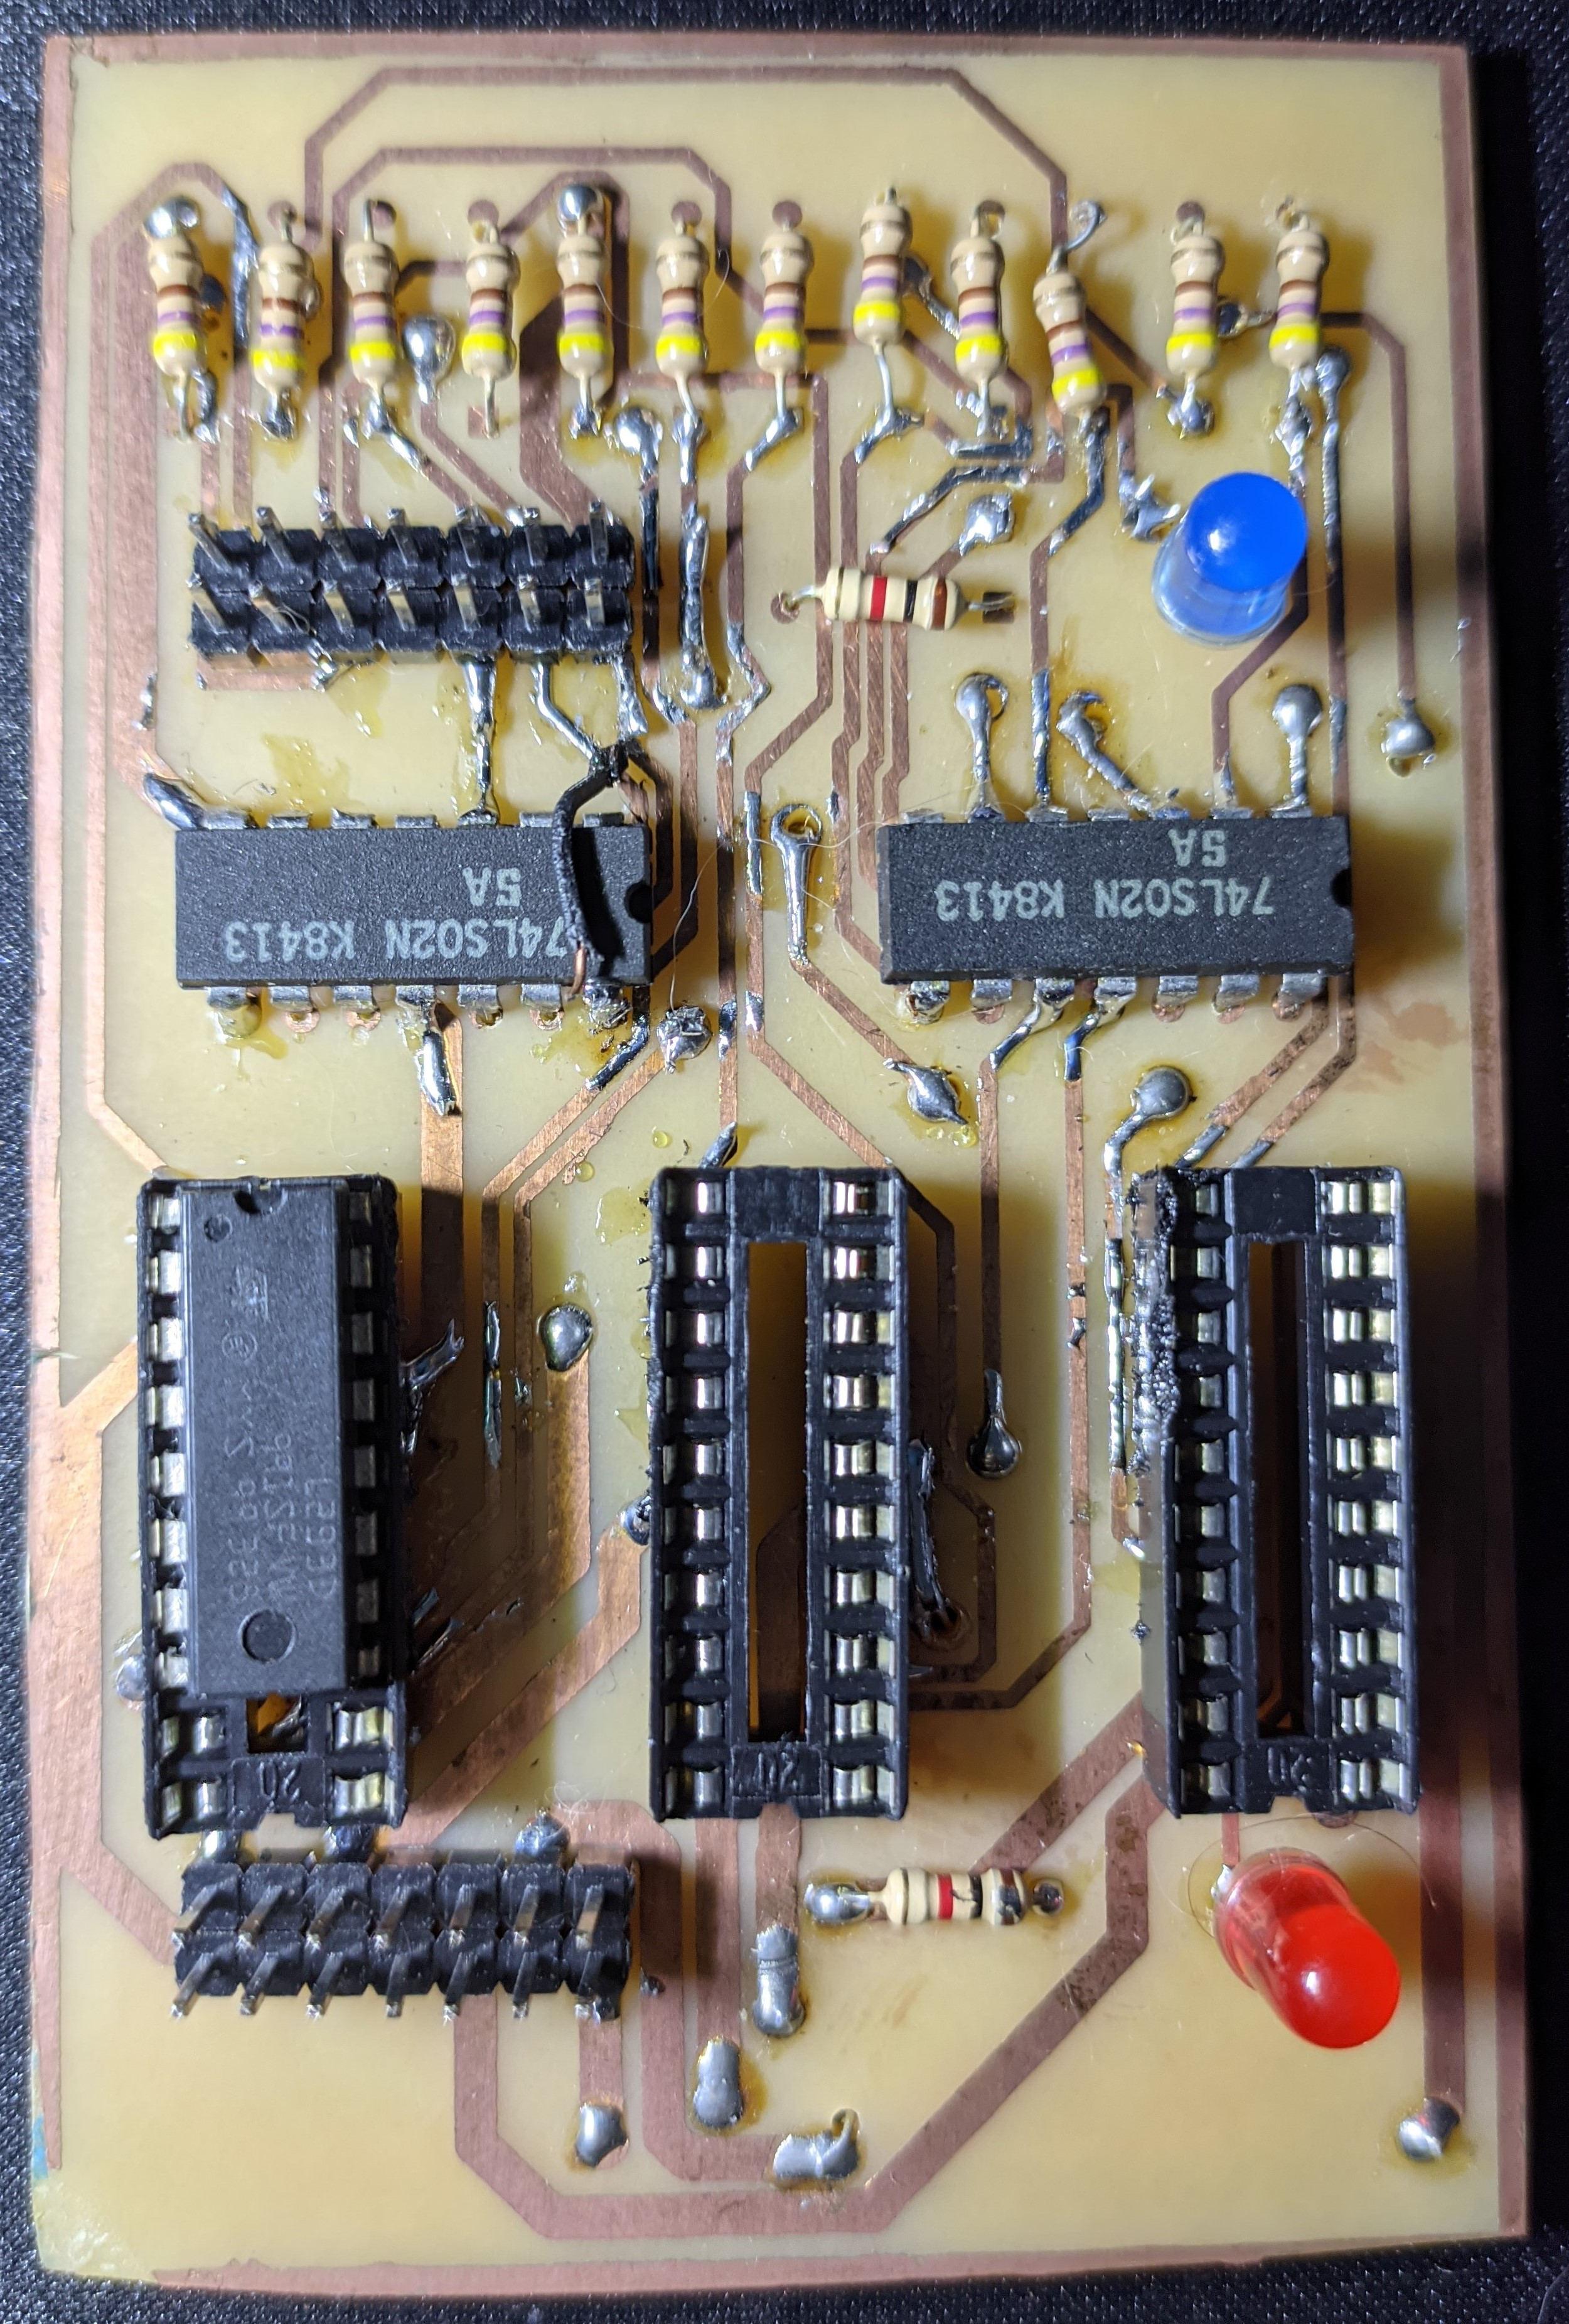
\includegraphics[keepaspectratio=true, width=0.9\linewidth]
            {img/placa-controle.jpg}
        \fonte{Do próprio autor}
        \label{fig:placaControle}
    \end{minipage}%    
\end{figure}

\section[Leitura das manetes]{Leitura das manetes}
\label{sec:leituraManetes}

Após a montagem da placa de controle, foi desenvolvido um \textit{software} com o microcontrolador para realizar a leitura dos dados das manetes.
Conforme descrito na subseção \ref{sub:maneteJogadores}, cada manete possui dois \textit{joysticks} com dois eixos e um botão cada.

Para realizar a leitura dos eixos dos \textit{joysticks}, foram utilizadas as entradas analógicas do microcontrolador.
Como o Arduino utiliza um conversor analógico-digital de 10 bits, os valores lidos variam de 0 a 1023.
Valores próximos de 512 representam a posição central do \textit{joystick}, enquanto valores próximos de 0 ou 1023 representam as posições extremas.
Para aprimorar a usabilidade da manete, foi implementada uma área de \textit{deadzone}, na qual o valor lido é considerado como zero, para evitar que o manipulador se movimente sem a intenção do usuário.

Para realizar a leitura do botão, foi utilizada uma entrada digital.
Esses botões possuem um \textit{pull-up} interno, o que significa que o valor lido é 1 quando o botão não está pressionado e 0 quando o botão está pressionado.

Os valores lidos são armazenados em uma variável, que é utilizada para realizar o controle do movimento do manipulador robótico.

\section[Cálculo da posição]{Cálculo da posição}
\label{sec:calculoPosicao}

Para calcular a posição do manipulador robótico, foi utilizado como base o \textit{software} desenvolvido anteriormente para ler os dados das manetes.

Para essa primeira parte do trabalho, o cálculo de posição foi feito de forma individual para cada junta.
Dessa forma, o usuário pode utilizar os 4 eixos dos \textit{joysticks} para controlar o manipulador robótico.
Além disso, o usuário pode utilizar o botão de cada manete para controlar a abertura e o fechamento da garra.

\section[Controle dos motores]{Controle dos motores}
\label{sec:controleMotores}

O controle dos motores foi incorporado no \textit{software} desenvolvido na subseção anterior, que realiza o cálculo da posição desejada das juntas.

Primeiramente foi implementada a leitura da posição atual de cada junta, utilizando as entradas analógicas do microcontrolador.
Os valores de 10 bits lidos pelo Arduino são convertidos para graus, utilizando como referência as faixas de movimento descritas nas tabelas \ref{tab:caracteristicasManipuladorMentor} e \ref{tab:caracteristicasManipuladorAzul}.

Depois disso, foi feita a implementação de um controlador para o manipulador.
Esse controlador é executado a cada 10ms, de acordo com a configuração da interrupção do \textit{timer} do Arduino.
Nessa interrupção, o microcontrolador calcula o erro entre a posição desejada e a posição atual de cada junta, com base nos valores lidos do manipulador e das manetes.
Em seguida, o valor de saída é calculado utilizando um algoritmo PID.
Esse algoritmo utiliza três constantes (Kp, Ki e Kd) e os valores do erro atual, da integral dos erros anteriores e da derivada do erro atual para calcular a saída.
Por fim, esse valor de saída é convertido em um valor de \textit{duty cycle}, e é utilizado para gerar o sinal PWM enviado para a placa de controle.

\chapter[Conclusões Preliminares]{Conclusões Preliminares}
\label{cap:conclusoes}

Durante o desenvolvimento do projeto, foi possível finalizar a placa de controle e um \textit{software} básico que permite o controle independente de cada junta.
Nessa primeira etapa de desenvolvimento, não foi possível implementar a lógica do jogo de Xadrez, tarefa que será realizada na próxima etapa.

O processo de produção da placa de controle foi mais demorado do que o inicialmente esperado, em parte pela necessidade de um cuidado especial para garantir que ambas as camadas estejam alinhadas.
Além disso, o processo de perfuração e soldagem da placa foi um pouco complicado e demorado.
Apesar disso, o resultado final foi satisfatório e a placa de controle apresenta um funcionamento adequado para o controle dos manipuladores.

O \textit{software} desenvolvido para o controle dos manipuladores, apesar de funcional, não facilita o controle deles.
Realizar o controle independente de cada junta é um processo complicado e pode provocar um desinteresse dos jogadores pelo produto desenvolvido.
Para a próxima etapa, esse \textit{software} será melhorado para que o controle dos manipuladores seja realizado apenas em duas dimensões de forma que o microcontrolador será responsável pelo cálculo dos ângulos das juntas.

A integração dos microcontroladores com o computador também será desenvolvida na próxima etapa do trabalho.
Essa integração será responsável por verificar se os movimentos realizados pelos jogadores são validos e por identificar quando um jogador ganhou ou perdeu o jogo.

% ----------------------------------------------------------








% ----------------------------------------------------------
% Finaliza a parte no bookmark do PDF
% para que se inicie o bookmark na raiz
% e adiciona espaço de parte no Sumário
% ----------------------------------------------------------
\phantompart







% ----------------------------------------------------------
% ELEMENTOS PÓS-TEXTUAIS
% ----------------------------------------------------------

%% Baseado no arquivo: 
%% abtex2-modelo-trabalho-academico.tex, v-1.9.6 laurocesar
%% by abnTeX2 group at http://www.abntex.net.br/ 
%% Adaptado para um modelo de TCC (Graduação)

\postextual
% ----------------------------------------------------------

% ----------------------------------------------------------
% Referências bibliográficas
% ----------------------------------------------------------
\bibliography{cefet_mg_decom_abntex2}

% ----------------------------------------------------------
% Glossário
% ----------------------------------------------------------
%
% Consulte o manual da classe abntex2 para orientações sobre o glossário.
%
%\glossary

% ----------------------------------------------------------
% Apêndices
% ----------------------------------------------------------

% ---
% Inicia os apêndices
% ---
\begin{apendicesenv}

% Imprime uma página indicando o início dos apêndices
\partapendices

% ----------------------------------------------------------
\chapter{Título do primeiro apêndice}
% ----------------------------------------------------------

Suspendisse sollicitudin risus et accumsan tempor. Orci varius natoque penatibus et magnis dis parturient montes, nascetur ridiculus mus. Mauris tempor malesuada ligula sed vehicula. Fusce porta magna a blandit aliquet. Nullam auctor tellus et augue lobortis suscipit. Nunc aliquet interdum nisl, at accumsan ante. Donec convallis arcu massa, eu malesuada ex tincidunt quis. Suspendisse turpis orci, auctor et egestas sit amet, ultrices a nisl. Ut interdum metus eu erat facilisis cursus. Maecenas sed dignissim odio, non tempor ipsum. Quisque luctus mi non molestie volutpat.

Class aptent taciti sociosqu ad litora torquent per conubia nostra, per inceptos himenaeos. Proin sed nulla auctor, tempor mauris nec, placerat justo. Vestibulum finibus aliquet ultricies. Nulla facilisi. Ut ante orci, interdum ac sodales vel, porttitor eu justo. Proin laoreet lacinia sapien, non suscipit libero bibendum sit amet. 

% ----------------------------------------------------------
\chapter{Outro Apêndice}
% ----------------------------------------------------------
Nulla facilisi. Ut ante orci, interdum ac sodales vel, porttitor eu justo. Proin laoreet lacinia sapien, non suscipit libero bibendum sit amet. Aliquam orci risus, venenatis et nibh eget, dictum imperdiet ligula. Suspendisse sollicitudin risus et accumsan tempor. Orci varius natoque penatibus et magnis dis parturient montes, nascetur ridiculus mus. Mauris tempor malesuada ligula sed vehicula. Fusce porta magna a blandit aliquet. Nullam auctor tellus et augue lobortis suscipit. Nunc aliquet interdum nisl, at accumsan ante. Donec convallis arcu massa, eu malesuada ex tincidunt quis. Suspendisse turpis orci, auctor et egestas sit amet, ultrices a nisl. Ut interdum metus eu erat facilisis cursus. Maecenas sed dignissim odio, non tempor ipsum. Quisque luctus mi non molestie volutpat.

Nulla facilisi. Ut ante orci, interdum ac sodales vel, porttitor eu justo. Proin laoreet lacinia sapien, non suscipit libero bibendum sit amet.Mauris dictum ante urna, at posuere nulla fermentum id. Proin fermentum odio at elit tristique faucibus. Praesent sit amet facilisis enim, id pulvinar quam. Sed dignissim sem quis tortor tincidunt, mattis blandit eros viverra. Class aptent taciti sociosqu ad litora torquent per conubia nostra, per inceptos himenaeos. Proin sed nulla auctor, tempor mauris nec, placerat justo. Vestibulum finibus aliquet ultricies.  

\end{apendicesenv}
% ---


% ----------------------------------------------------------
% Anexos
% ----------------------------------------------------------

% ---
% Inicia os anexos
% ---
\begin{anexosenv}

% Imprime uma página indicando o início dos anexos
\partanexos

% ---
\chapter{Este é o título do primeiro anexo}
% ---
 Lorem ipsum dolor sit amet, consectetur adipiscing elit. Cras a ultrices dolor. Pellentesque id ex neque. Aliquam orci risus, venenatis et nibh eget, dictum imperdiet ligula. Suspendisse sollicitudin risus et accumsan tempor. Orci varius natoque penatibus et magnis dis parturient montes, nascetur ridiculus mus. Mauris tempor malesuada ligula sed vehicula. Fusce porta magna a blandit aliquet. Nullam auctor tellus et augue lobortis suscipit. Nunc aliquet interdum nisl, at accumsan ante. Donec convallis arcu massa, eu malesuada ex tincidunt quis. Suspendisse turpis orci, auctor et egestas sit amet, ultrices a nisl. Ut interdum metus eu erat facilisis cursus. Maecenas sed dignissim odio, non tempor ipsum. Quisque luctus mi non molestie volutpat.

Mauris dictum ante urna, at posuere nulla fermentum id. Proin fermentum odio at elit tristique faucibus. Praesent sit amet facilisis enim, id pulvinar quam. Sed dignissim sem quis tortor tincidunt, mattis blandit eros viverra. Class aptent taciti sociosqu ad litora torquent per conubia nostra, per inceptos himenaeos. Proin sed nulla auctor, tempor mauris nec, placerat justo. Vestibulum finibus aliquet ultricies. Nulla facilisi. Ut ante orci, interdum ac sodales vel, porttitor eu justo. Proin laoreet lacinia sapien, non suscipit libero bibendum sit amet. 

% ---
\chapter{SEgundo título do segundo anexo}
% ---
Aliquam orci risus, venenatis et nibh eget, dictum imperdiet ligula. Suspendisse sollicitudin risus et accumsan tempor. Orci varius natoque penatibus et magnis dis parturient montes, nascetur ridiculus mus. Mauris tempor malesuada ligula sed vehicula. Fusce porta magna a blandit aliquet. Nullam auctor tellus et augue lobortis suscipit. Nunc aliquet interdum nisl, at accumsan ante. Donec convallis arcu massa, eu malesuada ex tincidunt quis. Suspendisse turpis orci, auctor et egestas sit amet, ultrices a nisl. Ut interdum metus eu erat facilisis cursus. Maecenas sed dignissim odio, non tempor ipsum. Quisque luctus mi non molestie volutpat.

Praesent sit amet facilisis enim, id pulvinar quam. Sed dignissim sem quis tortor tincidunt, mattis blandit eros viverra. Class aptent taciti sociosqu ad litora torquent per conubia nostra, per inceptos himenaeos. Proin sed nulla auctor, tempor mauris nec, placerat justo. Vestibulum finibus aliquet ultricies. Nulla facilisi. Ut ante orci, interdum ac sodales vel, porttitor eu justo. Proin laoreet lacinia sapien, non suscipit libero bibendum sit amet. 



\end{anexosenv}



\end{document}
